%************************************************
\chapter{Causal Hypotheses}
\label{chapter:causal_hypotheses}
%************************************************

\section{Representing Static Space}

Spatial arrangements of static symbols are created by the reflective
thinking layers.  Static symbols are not contained within the physical
layer, but these symbols are used to represent transitions from the
past to the future, which are in turn used to create relationships
between causes and effects that are used for planning.  Thinking
activities use these Spatial arrangements of symbols to think about
the given activities of the physical layer as well as planning in the
first-order reflective layer.

\section{Representing Simultaneities}

{\mbox{\autoref{figure:example_simultaneity}}} shows an example
simultaneity.
\begin{figure}
\center
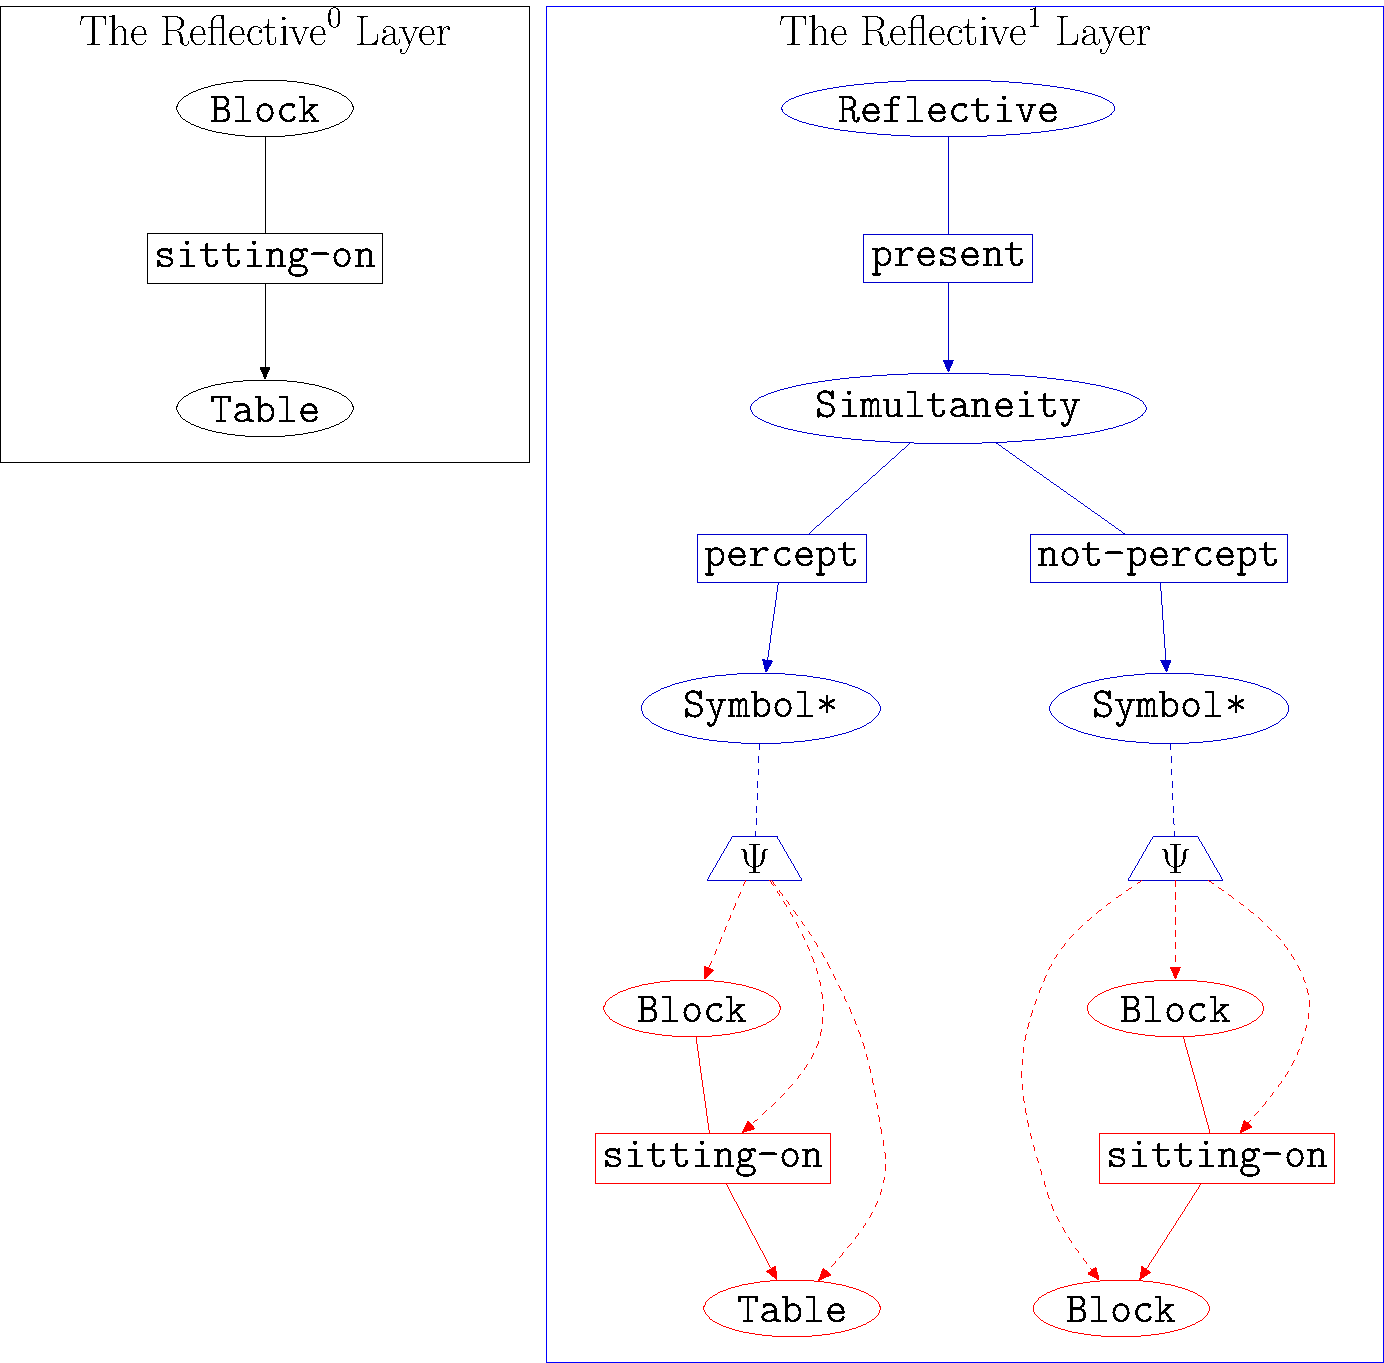
\includegraphics[width=10cm]{gfx/example_simultaneity}
\caption[Example simultaneity of positive and negative symbolic
  perceptions.]{Example simultaneity, $\text{\tt{simult}}_1^*$, of
  positive and negative symbolic perceptions, where the symbolic
  reference to physical activity, $x_1^*$, is perceived, while $x_2^*$
  is not.}
\label{figure:example_simultaneity}
\end{figure}

\section{Representing Transitions}

As {\mbox{\autoref{equation:define_symbol_referent_graph}}} states,
each reflective thinking layer can create symbolic references to
dynamic activities in the layers below as well as any other symbolic
activities in or below the symbolization activity.  Simultaneities and
transitions are the basis for representing concurrent and sequential
event knowledge.  It is a type of static Spatial arrangement between
static symbolic references.  Simultaneities and transitions can be
arranged into sequences back in time, forward in time, as well as
organizing time into binary trees for efficient recall.
\begin{figure}
\center
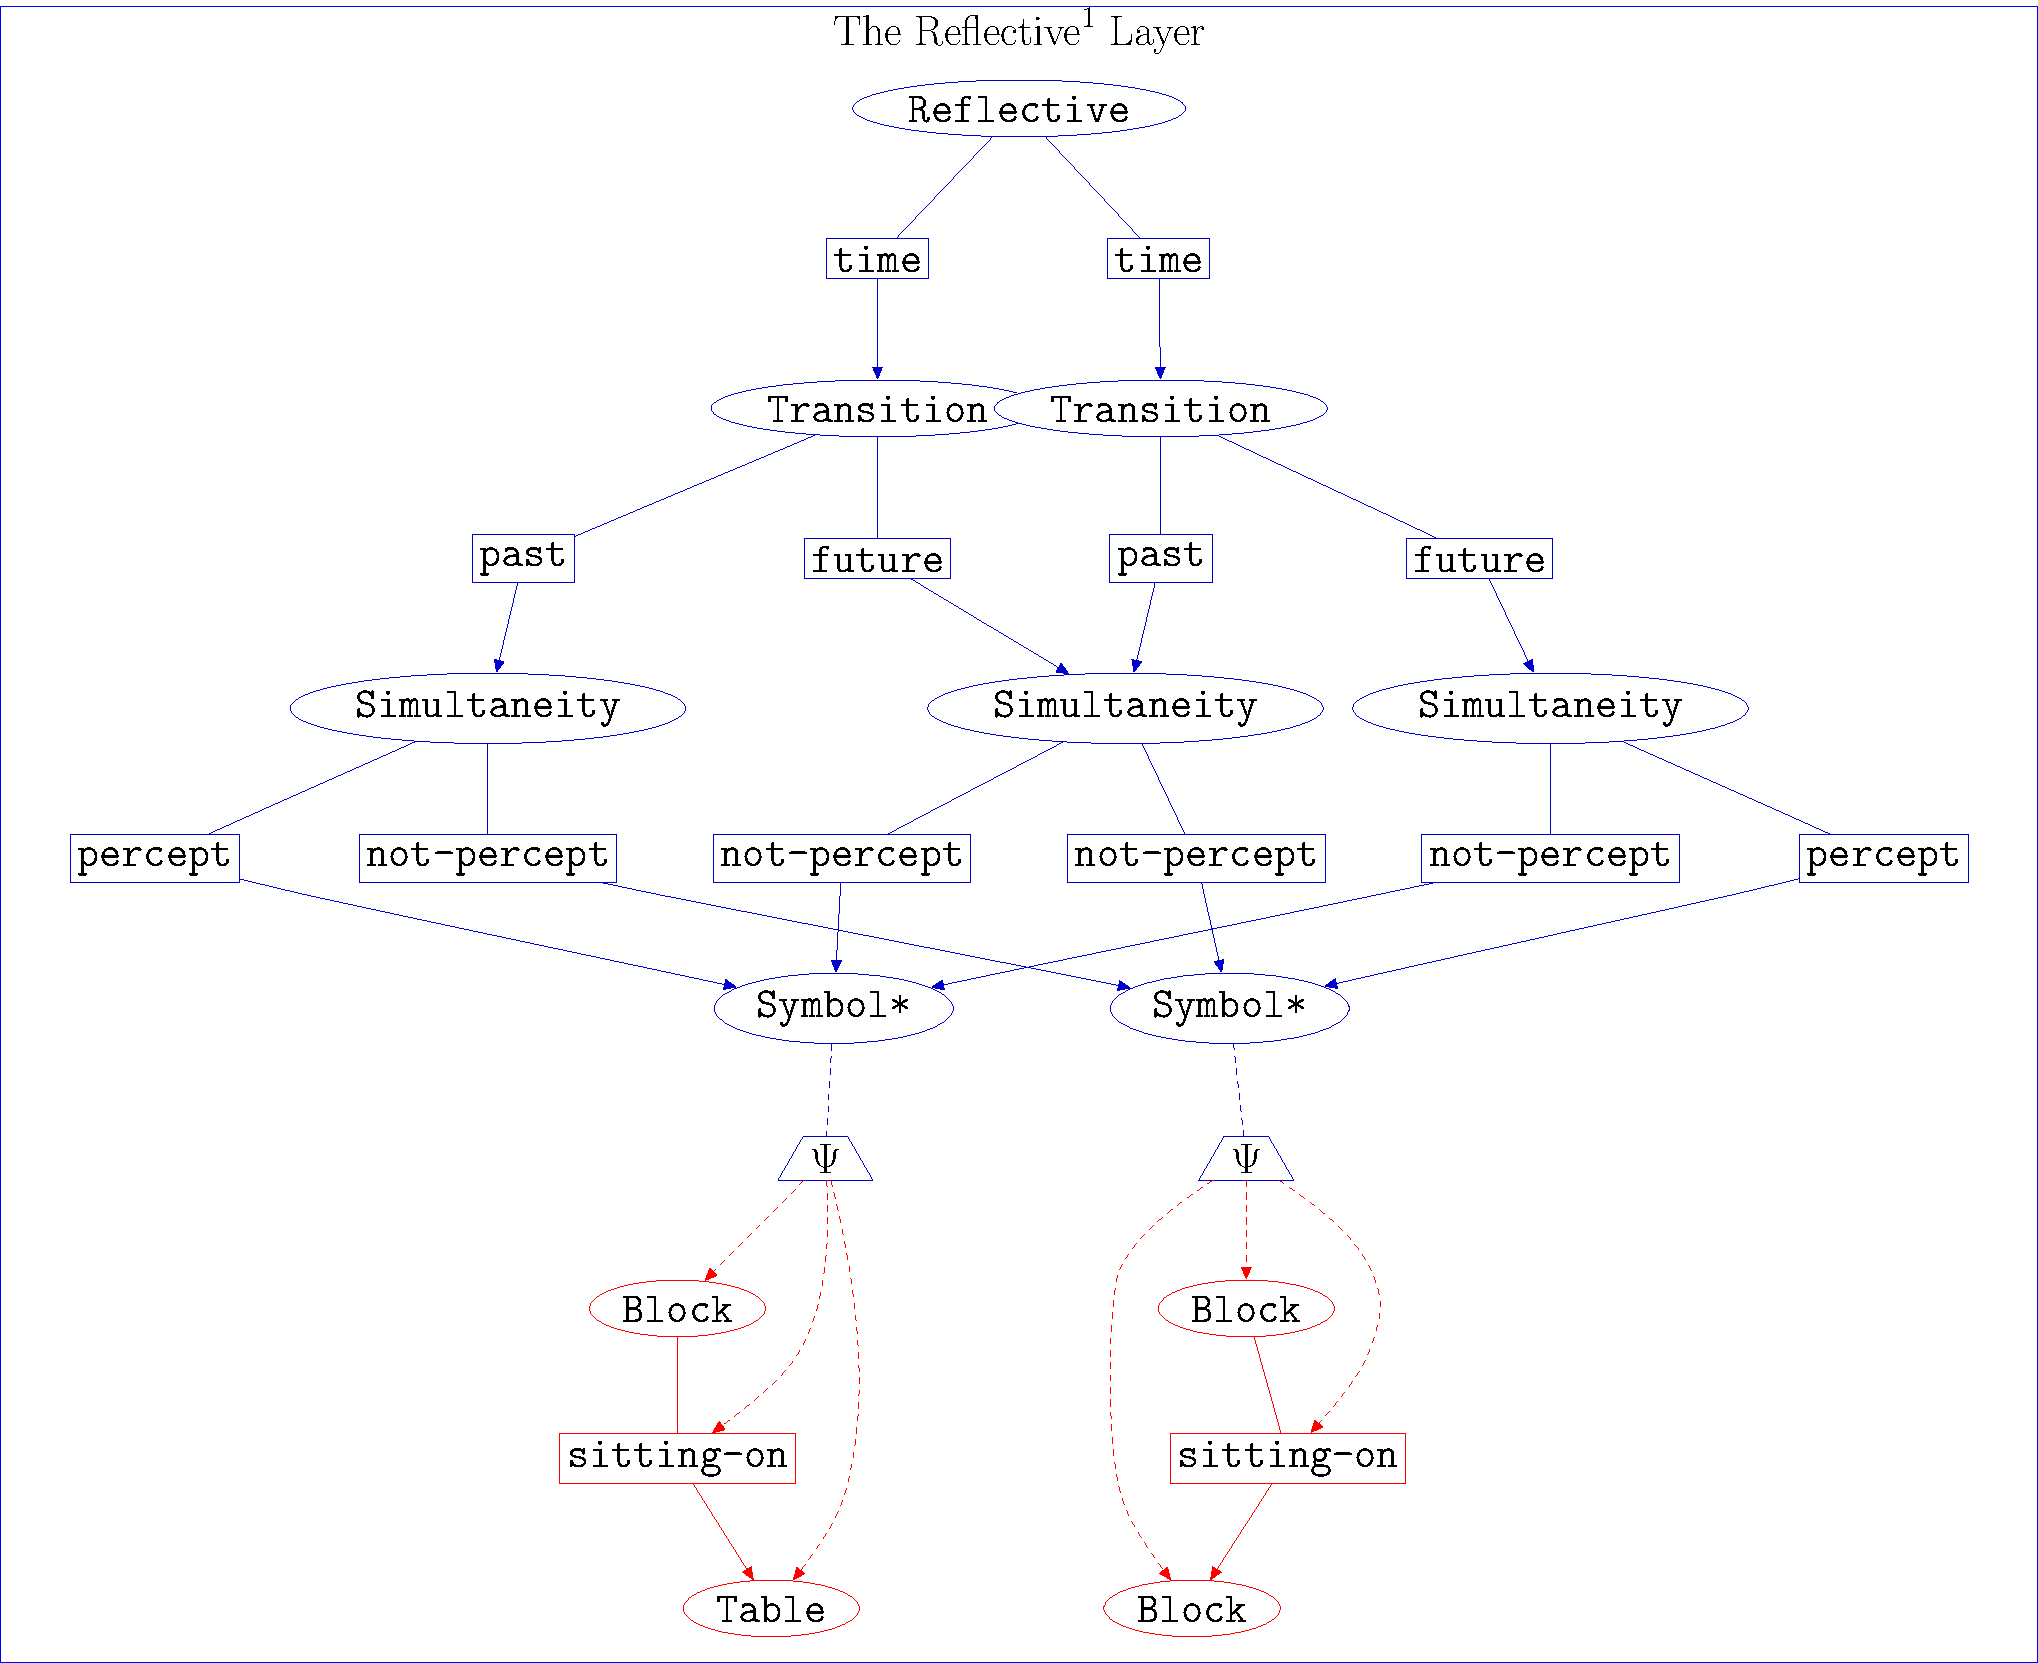
\includegraphics[width=12cm]{gfx/example_transition}
\caption[An example of a transition between simultaneities.]{An
  example of a transition between simultaneities,
  $\text{\tt{simult}}_1^*$ and $\text{\tt{simult}}_2^*$, which
  represent the transition between perceiving the first-order static
  symbolic reference, $x_1^*$, and then subsequently, $x_2^*$.}
\label{figure:example_transition}
\end{figure}

\section{Representing Transframes}

\begin{figure}
\center
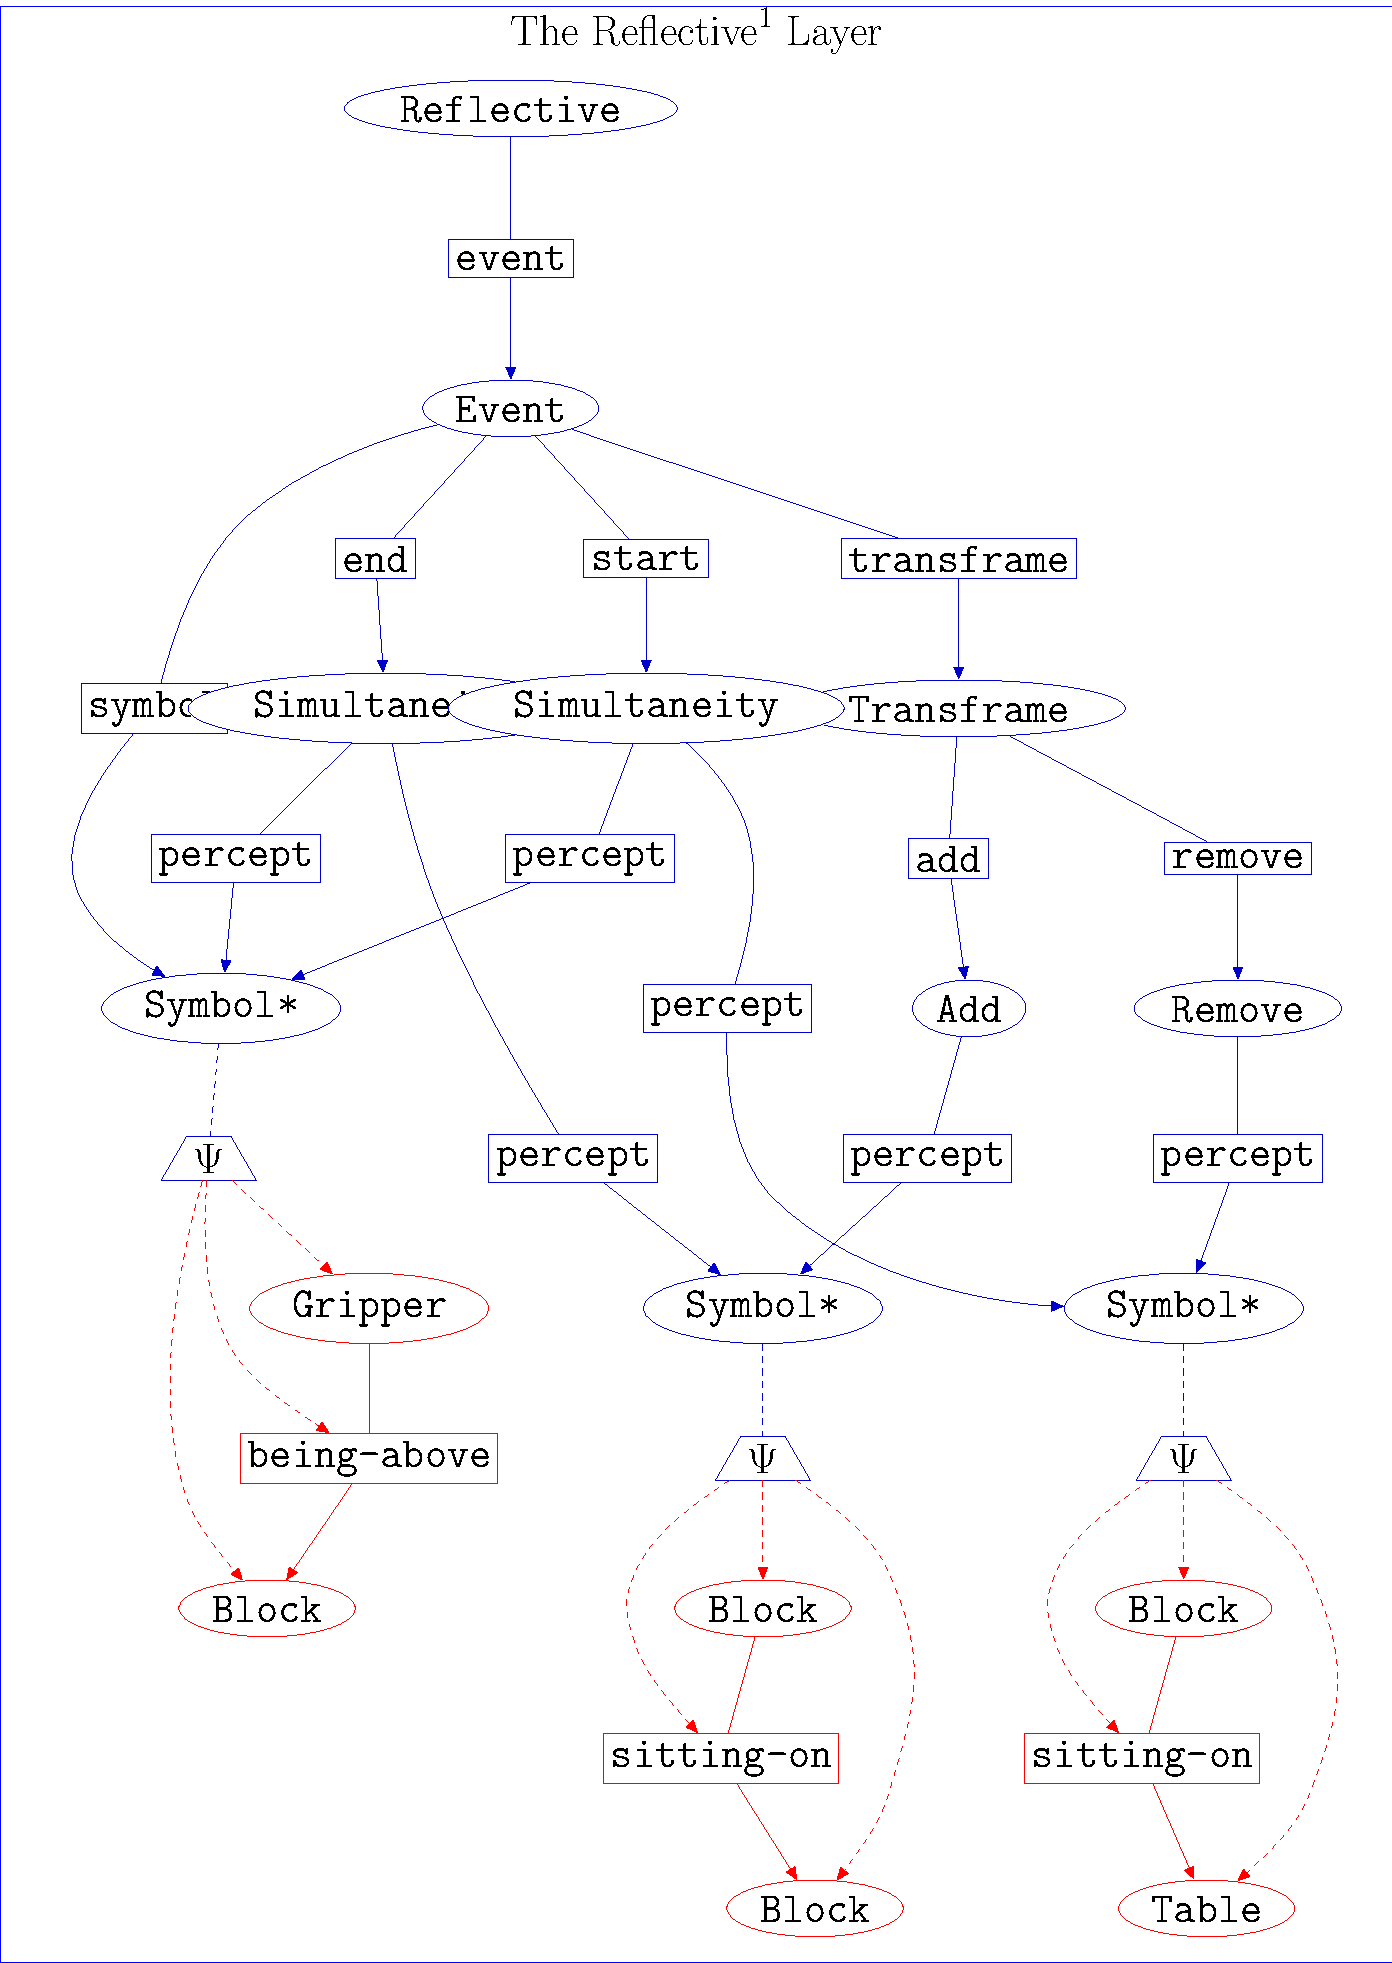
\includegraphics[width=12cm]{gfx/example_transframe}
\caption[An example of a transframe.]{An example of a transframe.}
\label{figure:example_transframe}
\end{figure}


\section{Representing Causal Hypotheses}

{\mbox{\autoref{figure:example_causal_hypothesis}}} shows an example
causal hypothesis, $h_1^*$, which introduces another symbolic
reference, $x_3^*$, to the physical layer, which is not shown.
\begin{figure}
\center
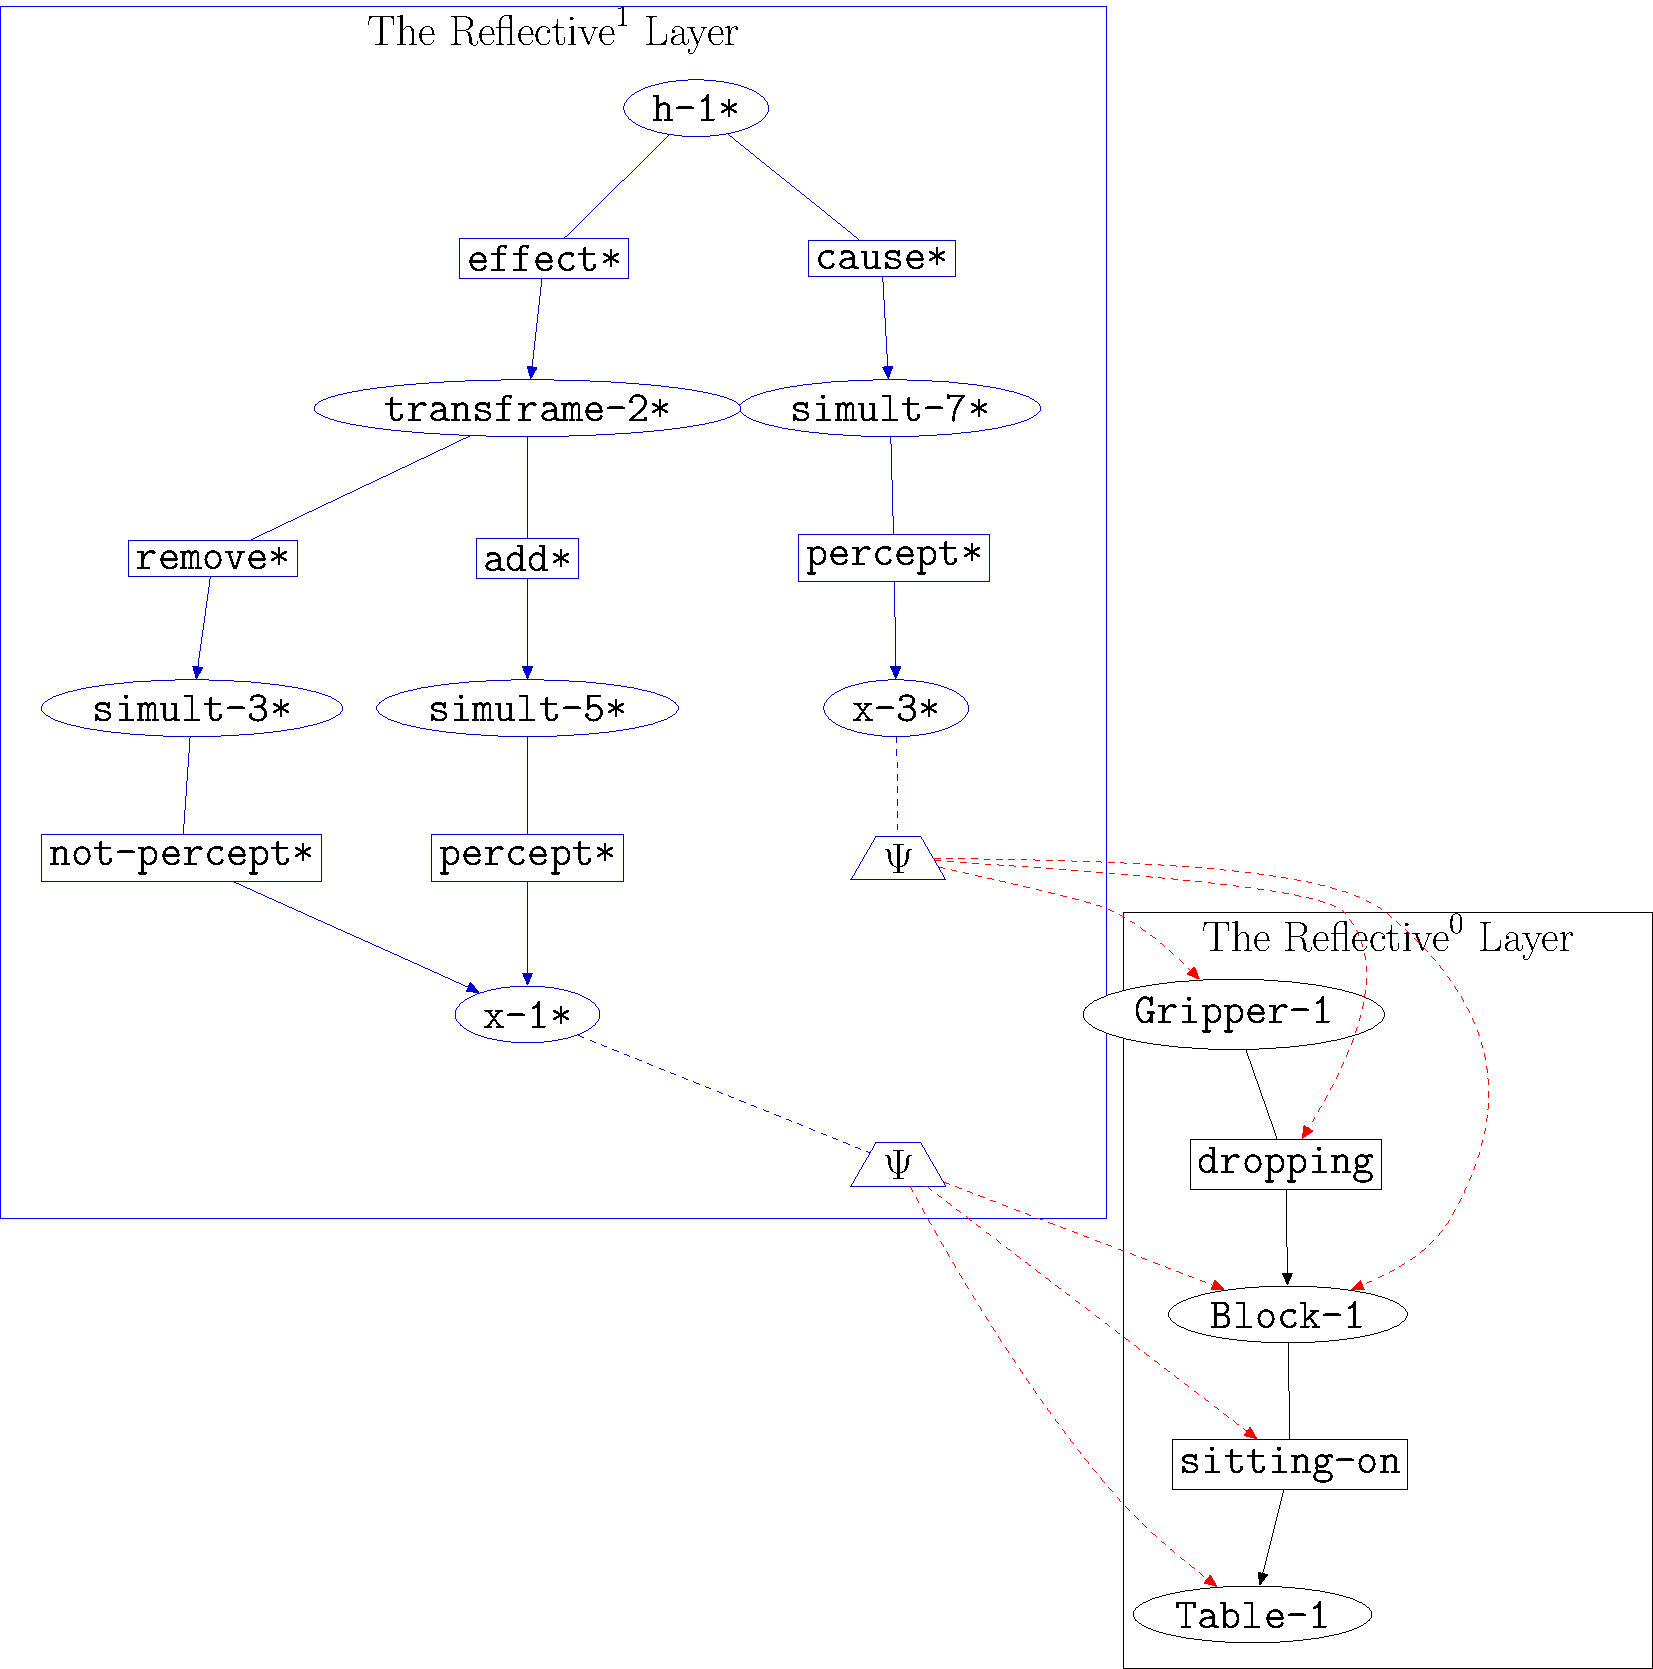
\includegraphics[width=12cm]{gfx/example_causal_hypothesis}
\caption[An example of a causal hypothesis.]{An example of a causal
  hypothesis, $h_1^*$, where the simultaneity,
  $\text{\tt{simult}}_3^*$, is hypothesized to be the cause of the
  transition, $\text{\tt{trans}}_1^*$.}
\label{figure:example_causal_hypothesis}
\end{figure}

\section{Representing Resources}

